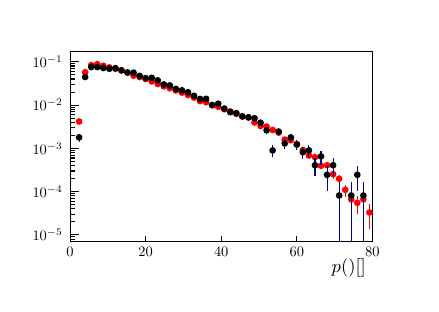
\begin{tikzpicture}
\pgfdeclareplotmark{cross} {
\pgfpathmoveto{\pgfpoint{-0.3\pgfplotmarksize}{\pgfplotmarksize}}
\pgfpathlineto{\pgfpoint{+0.3\pgfplotmarksize}{\pgfplotmarksize}}
\pgfpathlineto{\pgfpoint{+0.3\pgfplotmarksize}{0.3\pgfplotmarksize}}
\pgfpathlineto{\pgfpoint{+1\pgfplotmarksize}{0.3\pgfplotmarksize}}
\pgfpathlineto{\pgfpoint{+1\pgfplotmarksize}{-0.3\pgfplotmarksize}}
\pgfpathlineto{\pgfpoint{+0.3\pgfplotmarksize}{-0.3\pgfplotmarksize}}
\pgfpathlineto{\pgfpoint{+0.3\pgfplotmarksize}{-1.\pgfplotmarksize}}
\pgfpathlineto{\pgfpoint{-0.3\pgfplotmarksize}{-1.\pgfplotmarksize}}
\pgfpathlineto{\pgfpoint{-0.3\pgfplotmarksize}{-0.3\pgfplotmarksize}}
\pgfpathlineto{\pgfpoint{-1.\pgfplotmarksize}{-0.3\pgfplotmarksize}}
\pgfpathlineto{\pgfpoint{-1.\pgfplotmarksize}{0.3\pgfplotmarksize}}
\pgfpathlineto{\pgfpoint{-0.3\pgfplotmarksize}{0.3\pgfplotmarksize}}
\pgfpathclose
\pgfusepathqstroke
}
\pgfdeclareplotmark{cross*} {
\pgfpathmoveto{\pgfpoint{-0.3\pgfplotmarksize}{\pgfplotmarksize}}
\pgfpathlineto{\pgfpoint{+0.3\pgfplotmarksize}{\pgfplotmarksize}}
\pgfpathlineto{\pgfpoint{+0.3\pgfplotmarksize}{0.3\pgfplotmarksize}}
\pgfpathlineto{\pgfpoint{+1\pgfplotmarksize}{0.3\pgfplotmarksize}}
\pgfpathlineto{\pgfpoint{+1\pgfplotmarksize}{-0.3\pgfplotmarksize}}
\pgfpathlineto{\pgfpoint{+0.3\pgfplotmarksize}{-0.3\pgfplotmarksize}}
\pgfpathlineto{\pgfpoint{+0.3\pgfplotmarksize}{-1.\pgfplotmarksize}}
\pgfpathlineto{\pgfpoint{-0.3\pgfplotmarksize}{-1.\pgfplotmarksize}}
\pgfpathlineto{\pgfpoint{-0.3\pgfplotmarksize}{-0.3\pgfplotmarksize}}
\pgfpathlineto{\pgfpoint{-1.\pgfplotmarksize}{-0.3\pgfplotmarksize}}
\pgfpathlineto{\pgfpoint{-1.\pgfplotmarksize}{0.3\pgfplotmarksize}}
\pgfpathlineto{\pgfpoint{-0.3\pgfplotmarksize}{0.3\pgfplotmarksize}}
\pgfpathclose
\pgfusepathqfillstroke
}
\pgfdeclareplotmark{newstar} {
\pgfpathmoveto{\pgfqpoint{0pt}{\pgfplotmarksize}}
\pgfpathlineto{\pgfqpointpolar{44}{0.5\pgfplotmarksize}}
\pgfpathlineto{\pgfqpointpolar{18}{\pgfplotmarksize}}
\pgfpathlineto{\pgfqpointpolar{-20}{0.5\pgfplotmarksize}}
\pgfpathlineto{\pgfqpointpolar{-54}{\pgfplotmarksize}}
\pgfpathlineto{\pgfqpointpolar{-90}{0.5\pgfplotmarksize}}
\pgfpathlineto{\pgfqpointpolar{234}{\pgfplotmarksize}}
\pgfpathlineto{\pgfqpointpolar{198}{0.5\pgfplotmarksize}}
\pgfpathlineto{\pgfqpointpolar{162}{\pgfplotmarksize}}
\pgfpathlineto{\pgfqpointpolar{134}{0.5\pgfplotmarksize}}
\pgfpathclose
\pgfusepathqstroke
}
\pgfdeclareplotmark{newstar*} {
\pgfpathmoveto{\pgfqpoint{0pt}{\pgfplotmarksize}}
\pgfpathlineto{\pgfqpointpolar{44}{0.5\pgfplotmarksize}}
\pgfpathlineto{\pgfqpointpolar{18}{\pgfplotmarksize}}
\pgfpathlineto{\pgfqpointpolar{-20}{0.5\pgfplotmarksize}}
\pgfpathlineto{\pgfqpointpolar{-54}{\pgfplotmarksize}}
\pgfpathlineto{\pgfqpointpolar{-90}{0.5\pgfplotmarksize}}
\pgfpathlineto{\pgfqpointpolar{234}{\pgfplotmarksize}}
\pgfpathlineto{\pgfqpointpolar{198}{0.5\pgfplotmarksize}}
\pgfpathlineto{\pgfqpointpolar{162}{\pgfplotmarksize}}
\pgfpathlineto{\pgfqpointpolar{134}{0.5\pgfplotmarksize}}
\pgfpathclose
\pgfusepathqfillstroke
}
\definecolor{c}{rgb}{1,1,1};
\draw [color=c, fill=c] (0.1,3.20034) rectangle (4.9,6.21242);
\draw [color=c, fill=c] (0.58,3.50154) rectangle (4.42,5.91121);
\definecolor{c}{rgb}{0,0,0};
\draw [c] (0.58,3.50154) -- (0.58,5.91121) -- (4.42,5.91121) -- (4.42,3.50154) -- (0.58,3.50154);
\definecolor{c}{rgb}{1,0,0};
\draw [c] (0.6952,5.01563) -- (0.6952,5.0282);
\draw [c] (0.6952,5.0282) -- (0.6952,5.04014);
\draw [c] (0.6568,5.0282) -- (0.6952,5.0282);
\draw [c] (0.6952,5.0282) -- (0.7336,5.0282);
\foreach \P in {(0.6952,5.0282)}{\draw[mark options={color=c,fill=c},mark size=2.402402pt,mark=*,mark size=1pt] plot coordinates {\P};}
\draw [c] (0.772,5.65055) -- (0.772,5.65387);
\draw [c] (0.772,5.65387) -- (0.772,5.65715);
\draw [c] (0.7336,5.65387) -- (0.772,5.65387);
\draw [c] (0.772,5.65387) -- (0.8104,5.65387);
\foreach \P in {(0.772,5.65387)}{\draw[mark options={color=c,fill=c},mark size=2.402402pt,mark=*,mark size=1pt] plot coordinates {\P};}
\draw [c] (0.8488,5.74086) -- (0.8488,5.74361);
\draw [c] (0.8488,5.74361) -- (0.8488,5.74633);
\draw [c] (0.8104,5.74361) -- (0.8488,5.74361);
\draw [c] (0.8488,5.74361) -- (0.8872,5.74361);
\foreach \P in {(0.8488,5.74361)}{\draw[mark options={color=c,fill=c},mark size=2.402402pt,mark=*,mark size=1pt] plot coordinates {\P};}
\draw [c] (0.9256,5.75333) -- (0.9256,5.75601);
\draw [c] (0.9256,5.75601) -- (0.9256,5.75866);
\draw [c] (0.8872,5.75601) -- (0.9256,5.75601);
\draw [c] (0.9256,5.75601) -- (0.964,5.75601);
\foreach \P in {(0.9256,5.75601)}{\draw[mark options={color=c,fill=c},mark size=2.402402pt,mark=*,mark size=1pt] plot coordinates {\P};}
\draw [c] (1.0024,5.73281) -- (1.0024,5.7356);
\draw [c] (1.0024,5.7356) -- (1.0024,5.73837);
\draw [c] (0.964,5.7356) -- (1.0024,5.7356);
\draw [c] (1.0024,5.7356) -- (1.0408,5.7356);
\foreach \P in {(1.0024,5.7356)}{\draw[mark options={color=c,fill=c},mark size=2.402402pt,mark=*,mark size=1pt] plot coordinates {\P};}
\draw [c] (1.0792,5.71214) -- (1.0792,5.71506);
\draw [c] (1.0792,5.71506) -- (1.0792,5.71795);
\draw [c] (1.0408,5.71506) -- (1.0792,5.71506);
\draw [c] (1.0792,5.71506) -- (1.1176,5.71506);
\foreach \P in {(1.0792,5.71506)}{\draw[mark options={color=c,fill=c},mark size=2.402402pt,mark=*,mark size=1pt] plot coordinates {\P};}
\draw [c] (1.156,5.69412) -- (1.156,5.69715);
\draw [c] (1.156,5.69715) -- (1.156,5.70015);
\draw [c] (1.1176,5.69715) -- (1.156,5.69715);
\draw [c] (1.156,5.69715) -- (1.1944,5.69715);
\foreach \P in {(1.156,5.69715)}{\draw[mark options={color=c,fill=c},mark size=2.402402pt,mark=*,mark size=1pt] plot coordinates {\P};}
\draw [c] (1.2328,5.67455) -- (1.2328,5.67772);
\draw [c] (1.2328,5.67772) -- (1.2328,5.68084);
\draw [c] (1.1944,5.67772) -- (1.2328,5.67772);
\draw [c] (1.2328,5.67772) -- (1.2712,5.67772);
\foreach \P in {(1.2328,5.67772)}{\draw[mark options={color=c,fill=c},mark size=2.402402pt,mark=*,mark size=1pt] plot coordinates {\P};}
\draw [c] (1.3096,5.64468) -- (1.3096,5.64805);
\draw [c] (1.3096,5.64805) -- (1.3096,5.65137);
\draw [c] (1.2712,5.64805) -- (1.3096,5.64805);
\draw [c] (1.3096,5.64805) -- (1.348,5.64805);
\foreach \P in {(1.3096,5.64805)}{\draw[mark options={color=c,fill=c},mark size=2.402402pt,mark=*,mark size=1pt] plot coordinates {\P};}
\draw [c] (1.3864,5.60566) -- (1.3864,5.60931);
\draw [c] (1.3864,5.60931) -- (1.3864,5.61291);
\draw [c] (1.348,5.60931) -- (1.3864,5.60931);
\draw [c] (1.3864,5.60931) -- (1.4248,5.60931);
\foreach \P in {(1.3864,5.60931)}{\draw[mark options={color=c,fill=c},mark size=2.402402pt,mark=*,mark size=1pt] plot coordinates {\P};}
\draw [c] (1.4632,5.58877) -- (1.4632,5.59255);
\draw [c] (1.4632,5.59255) -- (1.4632,5.59628);
\draw [c] (1.4248,5.59255) -- (1.4632,5.59255);
\draw [c] (1.4632,5.59255) -- (1.5016,5.59255);
\foreach \P in {(1.4632,5.59255)}{\draw[mark options={color=c,fill=c},mark size=2.402402pt,mark=*,mark size=1pt] plot coordinates {\P};}
\draw [c] (1.54,5.56336) -- (1.54,5.56735);
\draw [c] (1.54,5.56735) -- (1.54,5.57127);
\draw [c] (1.5016,5.56735) -- (1.54,5.56735);
\draw [c] (1.54,5.56735) -- (1.5784,5.56735);
\foreach \P in {(1.54,5.56735)}{\draw[mark options={color=c,fill=c},mark size=2.402402pt,mark=*,mark size=1pt] plot coordinates {\P};}
\draw [c] (1.6168,5.53291) -- (1.6168,5.53717);
\draw [c] (1.6168,5.53717) -- (1.6168,5.54135);
\draw [c] (1.5784,5.53717) -- (1.6168,5.53717);
\draw [c] (1.6168,5.53717) -- (1.6552,5.53717);
\foreach \P in {(1.6168,5.53717)}{\draw[mark options={color=c,fill=c},mark size=2.402402pt,mark=*,mark size=1pt] plot coordinates {\P};}
\draw [c] (1.6936,5.49985) -- (1.6936,5.50441);
\draw [c] (1.6936,5.50441) -- (1.6936,5.50888);
\draw [c] (1.6552,5.50441) -- (1.6936,5.50441);
\draw [c] (1.6936,5.50441) -- (1.732,5.50441);
\foreach \P in {(1.6936,5.50441)}{\draw[mark options={color=c,fill=c},mark size=2.402402pt,mark=*,mark size=1pt] plot coordinates {\P};}
\draw [c] (1.7704,5.46945) -- (1.7704,5.47431);
\draw [c] (1.7704,5.47431) -- (1.7704,5.47907);
\draw [c] (1.732,5.47431) -- (1.7704,5.47431);
\draw [c] (1.7704,5.47431) -- (1.8088,5.47431);
\foreach \P in {(1.7704,5.47431)}{\draw[mark options={color=c,fill=c},mark size=2.402402pt,mark=*,mark size=1pt] plot coordinates {\P};}
\draw [c] (1.8472,5.44494) -- (1.8472,5.45006);
\draw [c] (1.8472,5.45006) -- (1.8472,5.45506);
\draw [c] (1.8088,5.45006) -- (1.8472,5.45006);
\draw [c] (1.8472,5.45006) -- (1.8856,5.45006);
\foreach \P in {(1.8472,5.45006)}{\draw[mark options={color=c,fill=c},mark size=2.402402pt,mark=*,mark size=1pt] plot coordinates {\P};}
\draw [c] (1.924,5.41617) -- (1.924,5.42161);
\draw [c] (1.924,5.42161) -- (1.924,5.42692);
\draw [c] (1.8856,5.42161) -- (1.924,5.42161);
\draw [c] (1.924,5.42161) -- (1.9624,5.42161);
\foreach \P in {(1.924,5.42161)}{\draw[mark options={color=c,fill=c},mark size=2.402402pt,mark=*,mark size=1pt] plot coordinates {\P};}
\draw [c] (2.0008,5.38861) -- (2.0008,5.39437);
\draw [c] (2.0008,5.39437) -- (2.0008,5.39999);
\draw [c] (1.9624,5.39437) -- (2.0008,5.39437);
\draw [c] (2.0008,5.39437) -- (2.0392,5.39437);
\foreach \P in {(2.0008,5.39437)}{\draw[mark options={color=c,fill=c},mark size=2.402402pt,mark=*,mark size=1pt] plot coordinates {\P};}
\draw [c] (2.0776,5.35794) -- (2.0776,5.36407);
\draw [c] (2.0776,5.36407) -- (2.0776,5.37006);
\draw [c] (2.0392,5.36407) -- (2.0776,5.36407);
\draw [c] (2.0776,5.36407) -- (2.116,5.36407);
\foreach \P in {(2.0776,5.36407)}{\draw[mark options={color=c,fill=c},mark size=2.402402pt,mark=*,mark size=1pt] plot coordinates {\P};}
\draw [c] (2.1544,5.32421) -- (2.1544,5.33079);
\draw [c] (2.1544,5.33079) -- (2.1544,5.3372);
\draw [c] (2.116,5.33079) -- (2.1544,5.33079);
\draw [c] (2.1544,5.33079) -- (2.1928,5.33079);
\foreach \P in {(2.1544,5.33079)}{\draw[mark options={color=c,fill=c},mark size=2.402402pt,mark=*,mark size=1pt] plot coordinates {\P};}
\draw [c] (2.2312,5.27897) -- (2.2312,5.28621);
\draw [c] (2.2312,5.28621) -- (2.2312,5.29324);
\draw [c] (2.1928,5.28621) -- (2.2312,5.28621);
\draw [c] (2.2312,5.28621) -- (2.2696,5.28621);
\foreach \P in {(2.2312,5.28621)}{\draw[mark options={color=c,fill=c},mark size=2.402402pt,mark=*,mark size=1pt] plot coordinates {\P};}
\draw [c] (2.308,5.26516) -- (2.308,5.27262);
\draw [c] (2.308,5.27262) -- (2.308,5.27984);
\draw [c] (2.2696,5.27262) -- (2.308,5.27262);
\draw [c] (2.308,5.27262) -- (2.3464,5.27262);
\foreach \P in {(2.308,5.27262)}{\draw[mark options={color=c,fill=c},mark size=2.402402pt,mark=*,mark size=1pt] plot coordinates {\P};}
\draw [c] (2.3848,5.22565) -- (2.3848,5.23374);
\draw [c] (2.3848,5.23374) -- (2.3848,5.24158);
\draw [c] (2.3464,5.23374) -- (2.3848,5.23374);
\draw [c] (2.3848,5.23374) -- (2.4232,5.23374);
\foreach \P in {(2.3848,5.23374)}{\draw[mark options={color=c,fill=c},mark size=2.402402pt,mark=*,mark size=1pt] plot coordinates {\P};}
\draw [c] (2.4616,5.20566) -- (2.4616,5.21411);
\draw [c] (2.4616,5.21411) -- (2.4616,5.22226);
\draw [c] (2.4232,5.21411) -- (2.4616,5.21411);
\draw [c] (2.4616,5.21411) -- (2.5,5.21411);
\foreach \P in {(2.4616,5.21411)}{\draw[mark options={color=c,fill=c},mark size=2.402402pt,mark=*,mark size=1pt] plot coordinates {\P};}
\draw [c] (2.5384,5.17437) -- (2.5384,5.18338);
\draw [c] (2.5384,5.18338) -- (2.5384,5.19207);
\draw [c] (2.5,5.18338) -- (2.5384,5.18338);
\draw [c] (2.5384,5.18338) -- (2.5768,5.18338);
\foreach \P in {(2.5384,5.18338)}{\draw[mark options={color=c,fill=c},mark size=2.402402pt,mark=*,mark size=1pt] plot coordinates {\P};}
\draw [c] (2.6152,5.14603) -- (2.6152,5.1556);
\draw [c] (2.6152,5.1556) -- (2.6152,5.1648);
\draw [c] (2.5768,5.1556) -- (2.6152,5.1556);
\draw [c] (2.6152,5.1556) -- (2.6536,5.1556);
\foreach \P in {(2.6152,5.1556)}{\draw[mark options={color=c,fill=c},mark size=2.402402pt,mark=*,mark size=1pt] plot coordinates {\P};}
\draw [c] (2.692,5.11434) -- (2.692,5.12457);
\draw [c] (2.692,5.12457) -- (2.692,5.13437);
\draw [c] (2.6536,5.12457) -- (2.692,5.12457);
\draw [c] (2.692,5.12457) -- (2.7304,5.12457);
\foreach \P in {(2.692,5.12457)}{\draw[mark options={color=c,fill=c},mark size=2.402402pt,mark=*,mark size=1pt] plot coordinates {\P};}
\draw [c] (2.7688,5.07984) -- (2.7688,5.09083);
\draw [c] (2.7688,5.09083) -- (2.7688,5.10133);
\draw [c] (2.7304,5.09083) -- (2.7688,5.09083);
\draw [c] (2.7688,5.09083) -- (2.8072,5.09083);
\foreach \P in {(2.7688,5.09083)}{\draw[mark options={color=c,fill=c},mark size=2.402402pt,mark=*,mark size=1pt] plot coordinates {\P};}
\draw [c] (2.8456,5.06767) -- (2.8456,5.07894);
\draw [c] (2.8456,5.07894) -- (2.8456,5.0897);
\draw [c] (2.8072,5.07894) -- (2.8456,5.07894);
\draw [c] (2.8456,5.07894) -- (2.884,5.07894);
\foreach \P in {(2.8456,5.07894)}{\draw[mark options={color=c,fill=c},mark size=2.402402pt,mark=*,mark size=1pt] plot coordinates {\P};}
\draw [c] (2.9224,5.00305) -- (2.9224,5.01596);
\draw [c] (2.9224,5.01596) -- (2.9224,5.0282);
\draw [c] (2.884,5.01596) -- (2.9224,5.01596);
\draw [c] (2.9224,5.01596) -- (2.9608,5.01596);
\foreach \P in {(2.9224,5.01596)}{\draw[mark options={color=c,fill=c},mark size=2.402402pt,mark=*,mark size=1pt] plot coordinates {\P};}
\draw [c] (2.9992,4.95676) -- (2.9992,4.97098);
\draw [c] (2.9992,4.97098) -- (2.9992,4.9844);
\draw [c] (2.9608,4.97098) -- (2.9992,4.97098);
\draw [c] (2.9992,4.97098) -- (3.0376,4.97098);
\foreach \P in {(2.9992,4.97098)}{\draw[mark options={color=c,fill=c},mark size=2.402402pt,mark=*,mark size=1pt] plot coordinates {\P};}
\draw [c] (3.076,4.94839) -- (3.076,4.96286);
\draw [c] (3.076,4.96286) -- (3.076,4.97651);
\draw [c] (3.0376,4.96286) -- (3.076,4.96286);
\draw [c] (3.076,4.96286) -- (3.1144,4.96286);
\foreach \P in {(3.076,4.96286)}{\draw[mark options={color=c,fill=c},mark size=2.402402pt,mark=*,mark size=1pt] plot coordinates {\P};}
\draw [c] (3.1528,4.90464) -- (3.1528,4.9205);
\draw [c] (3.1528,4.9205) -- (3.1528,4.93537);
\draw [c] (3.1144,4.9205) -- (3.1528,4.9205);
\draw [c] (3.1528,4.9205) -- (3.1912,4.9205);
\foreach \P in {(3.1528,4.9205)}{\draw[mark options={color=c,fill=c},mark size=2.402402pt,mark=*,mark size=1pt] plot coordinates {\P};}
\draw [c] (3.2296,4.86839) -- (3.2296,4.8855);
\draw [c] (3.2296,4.8855) -- (3.2296,4.90147);
\draw [c] (3.1912,4.8855) -- (3.2296,4.8855);
\draw [c] (3.2296,4.8855) -- (3.268,4.8855);
\foreach \P in {(3.2296,4.8855)}{\draw[mark options={color=c,fill=c},mark size=2.402402pt,mark=*,mark size=1pt] plot coordinates {\P};}
\draw [c] (3.3064,4.77754) -- (3.3064,4.79824);
\draw [c] (3.3064,4.79824) -- (3.3064,4.81728);
\draw [c] (3.268,4.79824) -- (3.3064,4.79824);
\draw [c] (3.3064,4.79824) -- (3.3448,4.79824);
\foreach \P in {(3.3064,4.79824)}{\draw[mark options={color=c,fill=c},mark size=2.402402pt,mark=*,mark size=1pt] plot coordinates {\P};}
\draw [c] (3.3832,4.76878) -- (3.3832,4.78986);
\draw [c] (3.3832,4.78986) -- (3.3832,4.80923);
\draw [c] (3.3448,4.78986) -- (3.3832,4.78986);
\draw [c] (3.3832,4.78986) -- (3.4216,4.78986);
\foreach \P in {(3.3832,4.78986)}{\draw[mark options={color=c,fill=c},mark size=2.402402pt,mark=*,mark size=1pt] plot coordinates {\P};}
\draw [c] (3.46,4.71954) -- (3.46,4.74291);
\draw [c] (3.46,4.74291) -- (3.46,4.76419);
\draw [c] (3.4216,4.74291) -- (3.46,4.74291);
\draw [c] (3.46,4.74291) -- (3.4984,4.74291);
\foreach \P in {(3.46,4.74291)}{\draw[mark options={color=c,fill=c},mark size=2.402402pt,mark=*,mark size=1pt] plot coordinates {\P};}
\draw [c] (3.5368,4.63732) -- (3.5368,4.66507);
\draw [c] (3.5368,4.66507) -- (3.5368,4.68993);
\draw [c] (3.4984,4.66507) -- (3.5368,4.66507);
\draw [c] (3.5368,4.66507) -- (3.5752,4.66507);
\foreach \P in {(3.5368,4.66507)}{\draw[mark options={color=c,fill=c},mark size=2.402402pt,mark=*,mark size=1pt] plot coordinates {\P};}
\draw [c] (3.6136,4.56303) -- (3.6136,4.59544);
\draw [c] (3.6136,4.59544) -- (3.6136,4.62398);
\draw [c] (3.5752,4.59544) -- (3.6136,4.59544);
\draw [c] (3.6136,4.59544) -- (3.652,4.59544);
\foreach \P in {(3.6136,4.59544)}{\draw[mark options={color=c,fill=c},mark size=2.402402pt,mark=*,mark size=1pt] plot coordinates {\P};}
\draw [c] (3.6904,4.54146) -- (3.6904,4.57537);
\draw [c] (3.6904,4.57537) -- (3.6904,4.60506);
\draw [c] (3.652,4.57537) -- (3.6904,4.57537);
\draw [c] (3.6904,4.57537) -- (3.7288,4.57537);
\foreach \P in {(3.6904,4.57537)}{\draw[mark options={color=c,fill=c},mark size=2.402402pt,mark=*,mark size=1pt] plot coordinates {\P};}
\draw [c] (3.7672,4.42217) -- (3.7672,4.46569);
\draw [c] (3.7672,4.46569) -- (3.7672,4.50248);
\draw [c] (3.7288,4.46569) -- (3.7672,4.46569);
\draw [c] (3.7672,4.46569) -- (3.8056,4.46569);
\foreach \P in {(3.7672,4.46569)}{\draw[mark options={color=c,fill=c},mark size=2.402402pt,mark=*,mark size=1pt] plot coordinates {\P};}
\draw [c] (3.844,4.42936) -- (3.844,4.47223);
\draw [c] (3.844,4.47223) -- (3.844,4.50856);
\draw [c] (3.8056,4.47223) -- (3.844,4.47223);
\draw [c] (3.844,4.47223) -- (3.8824,4.47223);
\foreach \P in {(3.844,4.47223)}{\draw[mark options={color=c,fill=c},mark size=2.402402pt,mark=*,mark size=1pt] plot coordinates {\P};}
\draw [c] (3.9208,4.30293) -- (3.9208,4.35875);
\draw [c] (3.9208,4.35875) -- (3.9208,4.40395);
\draw [c] (3.8824,4.35875) -- (3.9208,4.35875);
\draw [c] (3.9208,4.35875) -- (3.9592,4.35875);
\foreach \P in {(3.9208,4.35875)}{\draw[mark options={color=c,fill=c},mark size=2.402402pt,mark=*,mark size=1pt] plot coordinates {\P};}
\draw [c] (3.9976,4.23608) -- (3.9976,4.30024);
\draw [c] (3.9976,4.30024) -- (3.9976,4.35076);
\draw [c] (3.9592,4.30024) -- (3.9976,4.30024);
\draw [c] (3.9976,4.30024) -- (4.036,4.30024);
\foreach \P in {(3.9976,4.30024)}{\draw[mark options={color=c,fill=c},mark size=2.402402pt,mark=*,mark size=1pt] plot coordinates {\P};}
\draw [c] (4.0744,4.0692) -- (4.0744,4.15994);
\draw [c] (4.0744,4.15994) -- (4.0744,4.22552);
\draw [c] (4.036,4.15994) -- (4.0744,4.15994);
\draw [c] (4.0744,4.15994) -- (4.1128,4.15994);
\foreach \P in {(4.0744,4.15994)}{\draw[mark options={color=c,fill=c},mark size=2.402402pt,mark=*,mark size=1pt] plot coordinates {\P};}
\draw [c] (4.1512,3.91277) -- (4.1512,4.03801);
\draw [c] (4.1512,4.03801) -- (4.1512,4.11972);
\draw [c] (4.1128,4.03801) -- (4.1512,4.03801);
\draw [c] (4.1512,4.03801) -- (4.1896,4.03801);
\foreach \P in {(4.1512,4.03801)}{\draw[mark options={color=c,fill=c},mark size=2.402402pt,mark=*,mark size=1pt] plot coordinates {\P};}
\draw [c] (4.228,3.853) -- (4.228,3.99449);
\draw [c] (4.228,3.99449) -- (4.228,4.08272);
\draw [c] (4.1896,3.99449) -- (4.228,3.99449);
\draw [c] (4.228,3.99449) -- (4.2664,3.99449);
\foreach \P in {(4.228,3.99449)}{\draw[mark options={color=c,fill=c},mark size=2.402402pt,mark=*,mark size=1pt] plot coordinates {\P};}
\draw [c] (4.3048,3.91277) -- (4.3048,4.03801);
\draw [c] (4.3048,4.03801) -- (4.3048,4.11972);
\draw [c] (4.2664,4.03801) -- (4.3048,4.03801);
\draw [c] (4.3048,4.03801) -- (4.3432,4.03801);
\foreach \P in {(4.3048,4.03801)}{\draw[mark options={color=c,fill=c},mark size=2.402402pt,mark=*,mark size=1pt] plot coordinates {\P};}
\draw [c] (4.3816,3.66699) -- (4.3816,3.87256);
\draw [c] (4.3816,3.87256) -- (4.3816,3.98134);
\draw [c] (4.3432,3.87256) -- (4.3816,3.87256);
\draw [c] (4.3816,3.87256) -- (4.42,3.87256);
\foreach \P in {(4.3816,3.87256)}{\draw[mark options={color=c,fill=c},mark size=2.402402pt,mark=*,mark size=1pt] plot coordinates {\P};}
\definecolor{c}{rgb}{0,0,0};
\draw [c] (0.58,3.50154) -- (4.42,3.50154);
\draw [anchor= east] (4.42,3.16419) node[scale=0.672711, rotate=0]{$p(\kaon) [\mevc]$};
\draw [c] (0.58,3.57383) -- (0.58,3.50154);
\draw [c] (1.54,3.57383) -- (1.54,3.50154);
\draw [c] (2.5,3.57383) -- (2.5,3.50154);
\draw [c] (3.46,3.57383) -- (3.46,3.50154);
\draw [c] (4.42,3.57383) -- (4.42,3.50154);
\draw [anchor=base] (0.58,3.30877) node[scale=0.52322, rotate=0]{0};
\draw [anchor=base] (1.54,3.30877) node[scale=0.52322, rotate=0]{20};
\draw [anchor=base] (2.5,3.30877) node[scale=0.52322, rotate=0]{40};
\draw [anchor=base] (3.46,3.30877) node[scale=0.52322, rotate=0]{60};
\draw [anchor=base] (4.42,3.30877) node[scale=0.52322, rotate=0]{80};
\draw [c] (0.58,3.50154) -- (0.58,5.91121);
\draw [c] (0.6376,3.50214) -- (0.58,3.50214);
\draw [c] (0.6376,3.53402) -- (0.58,3.53402);
\draw [c] (0.6376,3.56213) -- (0.58,3.56213);
\draw [c] (0.6952,3.58728) -- (0.58,3.58728);
\draw [anchor= east] (0.54928,3.58728) node[scale=0.52322, rotate=0]{$10^{-5}$};
\draw [c] (0.6376,3.75273) -- (0.58,3.75273);
\draw [c] (0.6376,3.84951) -- (0.58,3.84951);
\draw [c] (0.6376,3.91818) -- (0.58,3.91818);
\draw [c] (0.6376,3.97144) -- (0.58,3.97144);
\draw [c] (0.6376,4.01496) -- (0.58,4.01496);
\draw [c] (0.6376,4.05175) -- (0.58,4.05175);
\draw [c] (0.6376,4.08363) -- (0.58,4.08363);
\draw [c] (0.6376,4.11174) -- (0.58,4.11174);
\draw [c] (0.6952,4.13689) -- (0.58,4.13689);
\draw [anchor= east] (0.54928,4.13689) node[scale=0.52322, rotate=0]{$10^{-4}$};
\draw [c] (0.6376,4.30234) -- (0.58,4.30234);
\draw [c] (0.6376,4.39912) -- (0.58,4.39912);
\draw [c] (0.6376,4.46779) -- (0.58,4.46779);
\draw [c] (0.6376,4.52105) -- (0.58,4.52105);
\draw [c] (0.6376,4.56457) -- (0.58,4.56457);
\draw [c] (0.6376,4.60136) -- (0.58,4.60136);
\draw [c] (0.6376,4.63324) -- (0.58,4.63324);
\draw [c] (0.6376,4.66135) -- (0.58,4.66135);
\draw [c] (0.6952,4.6865) -- (0.58,4.6865);
\draw [anchor= east] (0.54928,4.6865) node[scale=0.52322, rotate=0]{$10^{-3}$};
\draw [c] (0.6376,4.85195) -- (0.58,4.85195);
\draw [c] (0.6376,4.94873) -- (0.58,4.94873);
\draw [c] (0.6376,5.0174) -- (0.58,5.0174);
\draw [c] (0.6376,5.07066) -- (0.58,5.07066);
\draw [c] (0.6376,5.11418) -- (0.58,5.11418);
\draw [c] (0.6376,5.15097) -- (0.58,5.15097);
\draw [c] (0.6376,5.18285) -- (0.58,5.18285);
\draw [c] (0.6376,5.21096) -- (0.58,5.21096);
\draw [c] (0.6952,5.23611) -- (0.58,5.23611);
\draw [anchor= east] (0.54928,5.23611) node[scale=0.52322, rotate=0]{$10^{-2}$};
\draw [c] (0.6376,5.40156) -- (0.58,5.40156);
\draw [c] (0.6376,5.49834) -- (0.58,5.49834);
\draw [c] (0.6376,5.56701) -- (0.58,5.56701);
\draw [c] (0.6376,5.62027) -- (0.58,5.62027);
\draw [c] (0.6376,5.66379) -- (0.58,5.66379);
\draw [c] (0.6376,5.70058) -- (0.58,5.70058);
\draw [c] (0.6376,5.73246) -- (0.58,5.73246);
\draw [c] (0.6376,5.76057) -- (0.58,5.76057);
\draw [c] (0.6952,5.78572) -- (0.58,5.78572);
\draw [anchor= east] (0.54928,5.78572) node[scale=0.52322, rotate=0]{$10^{-1}$};
\definecolor{c}{rgb}{0,0,0.6};
\draw [c] (0.6952,4.76891) -- (0.6952,4.82614);
\draw [c] (0.6952,4.82614) -- (0.6952,4.87227);
\draw [c] (0.6568,4.82614) -- (0.6952,4.82614);
\draw [c] (0.6952,4.82614) -- (0.7336,4.82614);
\definecolor{c}{rgb}{0,0,0};
\foreach \P in {(0.6952,4.82614)}{\draw[mark options={color=c,fill=c},mark size=2.402402pt,mark=*,mark size=1pt] plot coordinates {\P};}
\definecolor{c}{rgb}{0,0,0.6};
\draw [c] (0.772,5.58273) -- (0.772,5.59316);
\draw [c] (0.772,5.59316) -- (0.772,5.60315);
\draw [c] (0.7336,5.59316) -- (0.772,5.59316);
\draw [c] (0.772,5.59316) -- (0.8104,5.59316);
\definecolor{c}{rgb}{0,0,0};
\foreach \P in {(0.772,5.59316)}{\draw[mark options={color=c,fill=c},mark size=2.402402pt,mark=*,mark size=1pt] plot coordinates {\P};}
\definecolor{c}{rgb}{0,0,0.6};
\draw [c] (0.8488,5.71136) -- (0.8488,5.71933);
\draw [c] (0.8488,5.71933) -- (0.8488,5.72704);
\draw [c] (0.8104,5.71933) -- (0.8488,5.71933);
\draw [c] (0.8488,5.71933) -- (0.8872,5.71933);
\definecolor{c}{rgb}{0,0,0};
\foreach \P in {(0.8488,5.71933)}{\draw[mark options={color=c,fill=c},mark size=2.402402pt,mark=*,mark size=1pt] plot coordinates {\P};}
\definecolor{c}{rgb}{0,0,0.6};
\draw [c] (0.9256,5.71136) -- (0.9256,5.71933);
\draw [c] (0.9256,5.71933) -- (0.9256,5.72704);
\draw [c] (0.8872,5.71933) -- (0.9256,5.71933);
\draw [c] (0.9256,5.71933) -- (0.964,5.71933);
\definecolor{c}{rgb}{0,0,0};
\foreach \P in {(0.9256,5.71933)}{\draw[mark options={color=c,fill=c},mark size=2.402402pt,mark=*,mark size=1pt] plot coordinates {\P};}
\definecolor{c}{rgb}{0,0,0.6};
\draw [c] (1.0024,5.69874) -- (1.0024,5.70692);
\draw [c] (1.0024,5.70692) -- (1.0024,5.71483);
\draw [c] (0.964,5.70692) -- (1.0024,5.70692);
\draw [c] (1.0024,5.70692) -- (1.0408,5.70692);
\definecolor{c}{rgb}{0,0,0};
\foreach \P in {(1.0024,5.70692)}{\draw[mark options={color=c,fill=c},mark size=2.402402pt,mark=*,mark size=1pt] plot coordinates {\P};}
\definecolor{c}{rgb}{0,0,0.6};
\draw [c] (1.0792,5.68918) -- (1.0792,5.69753);
\draw [c] (1.0792,5.69753) -- (1.0792,5.70559);
\draw [c] (1.0408,5.69753) -- (1.0792,5.69753);
\draw [c] (1.0792,5.69753) -- (1.1176,5.69753);
\definecolor{c}{rgb}{0,0,0};
\foreach \P in {(1.0792,5.69753)}{\draw[mark options={color=c,fill=c},mark size=2.402402pt,mark=*,mark size=1pt] plot coordinates {\P};}
\definecolor{c}{rgb}{0,0,0.6};
\draw [c] (1.156,5.6968) -- (1.156,5.70502);
\draw [c] (1.156,5.70502) -- (1.156,5.71296);
\draw [c] (1.1176,5.70502) -- (1.156,5.70502);
\draw [c] (1.156,5.70502) -- (1.1944,5.70502);
\definecolor{c}{rgb}{0,0,0};
\foreach \P in {(1.156,5.70502)}{\draw[mark options={color=c,fill=c},mark size=2.402402pt,mark=*,mark size=1pt] plot coordinates {\P};}
\definecolor{c}{rgb}{0,0,0.6};
\draw [c] (1.2328,5.6679) -- (1.2328,5.67663);
\draw [c] (1.2328,5.67663) -- (1.2328,5.68505);
\draw [c] (1.1944,5.67663) -- (1.2328,5.67663);
\draw [c] (1.2328,5.67663) -- (1.2712,5.67663);
\definecolor{c}{rgb}{0,0,0};
\foreach \P in {(1.2328,5.67663)}{\draw[mark options={color=c,fill=c},mark size=2.402402pt,mark=*,mark size=1pt] plot coordinates {\P};}
\definecolor{c}{rgb}{0,0,0.6};
\draw [c] (1.3096,5.64109) -- (1.3096,5.65032);
\draw [c] (1.3096,5.65032) -- (1.3096,5.6592);
\draw [c] (1.2712,5.65032) -- (1.3096,5.65032);
\draw [c] (1.3096,5.65032) -- (1.348,5.65032);
\definecolor{c}{rgb}{0,0,0};
\foreach \P in {(1.3096,5.65032)}{\draw[mark options={color=c,fill=c},mark size=2.402402pt,mark=*,mark size=1pt] plot coordinates {\P};}
\definecolor{c}{rgb}{0,0,0.6};
\draw [c] (1.3864,5.63862) -- (1.3864,5.6479);
\draw [c] (1.3864,5.6479) -- (1.3864,5.65683);
\draw [c] (1.348,5.6479) -- (1.3864,5.6479);
\draw [c] (1.3864,5.6479) -- (1.4248,5.6479);
\definecolor{c}{rgb}{0,0,0};
\foreach \P in {(1.3864,5.6479)}{\draw[mark options={color=c,fill=c},mark size=2.402402pt,mark=*,mark size=1pt] plot coordinates {\P};}
\definecolor{c}{rgb}{0,0,0.6};
\draw [c] (1.4632,5.59702) -- (1.4632,5.60714);
\draw [c] (1.4632,5.60714) -- (1.4632,5.61685);
\draw [c] (1.4248,5.60714) -- (1.4632,5.60714);
\draw [c] (1.4632,5.60714) -- (1.5016,5.60714);
\definecolor{c}{rgb}{0,0,0};
\foreach \P in {(1.4632,5.60714)}{\draw[mark options={color=c,fill=c},mark size=2.402402pt,mark=*,mark size=1pt] plot coordinates {\P};}
\definecolor{c}{rgb}{0,0,0.6};
\draw [c] (1.54,5.56754) -- (1.54,5.5783);
\draw [c] (1.54,5.5783) -- (1.54,5.58861);
\draw [c] (1.5016,5.5783) -- (1.54,5.5783);
\draw [c] (1.54,5.5783) -- (1.5784,5.5783);
\definecolor{c}{rgb}{0,0,0};
\foreach \P in {(1.54,5.5783)}{\draw[mark options={color=c,fill=c},mark size=2.402402pt,mark=*,mark size=1pt] plot coordinates {\P};}
\definecolor{c}{rgb}{0,0,0.6};
\draw [c] (1.6168,5.57178) -- (1.6168,5.58245);
\draw [c] (1.6168,5.58245) -- (1.6168,5.59266);
\draw [c] (1.5784,5.58245) -- (1.6168,5.58245);
\draw [c] (1.6168,5.58245) -- (1.6552,5.58245);
\definecolor{c}{rgb}{0,0,0};
\foreach \P in {(1.6168,5.58245)}{\draw[mark options={color=c,fill=c},mark size=2.402402pt,mark=*,mark size=1pt] plot coordinates {\P};}
\definecolor{c}{rgb}{0,0,0.6};
\draw [c] (1.6936,5.53881) -- (1.6936,5.55025);
\draw [c] (1.6936,5.55025) -- (1.6936,5.56116);
\draw [c] (1.6552,5.55025) -- (1.6936,5.55025);
\draw [c] (1.6936,5.55025) -- (1.732,5.55025);
\definecolor{c}{rgb}{0,0,0};
\foreach \P in {(1.6936,5.55025)}{\draw[mark options={color=c,fill=c},mark size=2.402402pt,mark=*,mark size=1pt] plot coordinates {\P};}
\definecolor{c}{rgb}{0,0,0.6};
\draw [c] (1.7704,5.48577) -- (1.7704,5.49855);
\draw [c] (1.7704,5.49855) -- (1.7704,5.51068);
\draw [c] (1.732,5.49855) -- (1.7704,5.49855);
\draw [c] (1.7704,5.49855) -- (1.8088,5.49855);
\definecolor{c}{rgb}{0,0,0};
\foreach \P in {(1.7704,5.49855)}{\draw[mark options={color=c,fill=c},mark size=2.402402pt,mark=*,mark size=1pt] plot coordinates {\P};}
\definecolor{c}{rgb}{0,0,0.6};
\draw [c] (1.8472,5.47276) -- (1.8472,5.48589);
\draw [c] (1.8472,5.48589) -- (1.8472,5.49834);
\draw [c] (1.8088,5.48589) -- (1.8472,5.48589);
\draw [c] (1.8472,5.48589) -- (1.8856,5.48589);
\definecolor{c}{rgb}{0,0,0};
\foreach \P in {(1.8472,5.48589)}{\draw[mark options={color=c,fill=c},mark size=2.402402pt,mark=*,mark size=1pt] plot coordinates {\P};}
\definecolor{c}{rgb}{0,0,0.6};
\draw [c] (1.924,5.42725) -- (1.924,5.44169);
\draw [c] (1.924,5.44169) -- (1.924,5.45531);
\draw [c] (1.8856,5.44169) -- (1.924,5.44169);
\draw [c] (1.924,5.44169) -- (1.9624,5.44169);
\definecolor{c}{rgb}{0,0,0};
\foreach \P in {(1.924,5.44169)}{\draw[mark options={color=c,fill=c},mark size=2.402402pt,mark=*,mark size=1pt] plot coordinates {\P};}
\definecolor{c}{rgb}{0,0,0.6};
\draw [c] (2.0008,5.40873) -- (2.0008,5.42375);
\draw [c] (2.0008,5.42375) -- (2.0008,5.43788);
\draw [c] (1.9624,5.42375) -- (2.0008,5.42375);
\draw [c] (2.0008,5.42375) -- (2.0392,5.42375);
\definecolor{c}{rgb}{0,0,0};
\foreach \P in {(2.0008,5.42375)}{\draw[mark options={color=c,fill=c},mark size=2.402402pt,mark=*,mark size=1pt] plot coordinates {\P};}
\definecolor{c}{rgb}{0,0,0.6};
\draw [c] (2.0776,5.38366) -- (2.0776,5.39949);
\draw [c] (2.0776,5.39949) -- (2.0776,5.41433);
\draw [c] (2.0392,5.39949) -- (2.0776,5.39949);
\draw [c] (2.0776,5.39949) -- (2.116,5.39949);
\definecolor{c}{rgb}{0,0,0};
\foreach \P in {(2.0776,5.39949)}{\draw[mark options={color=c,fill=c},mark size=2.402402pt,mark=*,mark size=1pt] plot coordinates {\P};}
\definecolor{c}{rgb}{0,0,0.6};
\draw [c] (2.1544,5.33673) -- (2.1544,5.35419);
\draw [c] (2.1544,5.35419) -- (2.1544,5.37046);
\draw [c] (2.116,5.35419) -- (2.1544,5.35419);
\draw [c] (2.1544,5.35419) -- (2.1928,5.35419);
\definecolor{c}{rgb}{0,0,0};
\foreach \P in {(2.1544,5.35419)}{\draw[mark options={color=c,fill=c},mark size=2.402402pt,mark=*,mark size=1pt] plot coordinates {\P};}
\definecolor{c}{rgb}{0,0,0.6};
\draw [c] (2.2312,5.29516) -- (2.2312,5.31421);
\draw [c] (2.2312,5.31421) -- (2.2312,5.33185);
\draw [c] (2.1928,5.31421) -- (2.2312,5.31421);
\draw [c] (2.2312,5.31421) -- (2.2696,5.31421);
\definecolor{c}{rgb}{0,0,0};
\foreach \P in {(2.2312,5.31421)}{\draw[mark options={color=c,fill=c},mark size=2.402402pt,mark=*,mark size=1pt] plot coordinates {\P};}
\definecolor{c}{rgb}{0,0,0.6};
\draw [c] (2.308,5.29662) -- (2.308,5.31561);
\draw [c] (2.308,5.31561) -- (2.308,5.3332);
\draw [c] (2.2696,5.31561) -- (2.308,5.31561);
\draw [c] (2.308,5.31561) -- (2.3464,5.31561);
\definecolor{c}{rgb}{0,0,0};
\foreach \P in {(2.308,5.31561)}{\draw[mark options={color=c,fill=c},mark size=2.402402pt,mark=*,mark size=1pt] plot coordinates {\P};}
\definecolor{c}{rgb}{0,0,0.6};
\draw [c] (2.3848,5.21441) -- (2.3848,5.23696);
\draw [c] (2.3848,5.23696) -- (2.3848,5.25757);
\draw [c] (2.3464,5.23696) -- (2.3848,5.23696);
\draw [c] (2.3848,5.23696) -- (2.4232,5.23696);
\definecolor{c}{rgb}{0,0,0};
\foreach \P in {(2.3848,5.23696)}{\draw[mark options={color=c,fill=c},mark size=2.402402pt,mark=*,mark size=1pt] plot coordinates {\P};}
\definecolor{c}{rgb}{0,0,0.6};
\draw [c] (2.4616,5.23208) -- (2.4616,5.25382);
\draw [c] (2.4616,5.25382) -- (2.4616,5.27374);
\draw [c] (2.4232,5.25382) -- (2.4616,5.25382);
\draw [c] (2.4616,5.25382) -- (2.5,5.25382);
\definecolor{c}{rgb}{0,0,0};
\foreach \P in {(2.4616,5.25382)}{\draw[mark options={color=c,fill=c},mark size=2.402402pt,mark=*,mark size=1pt] plot coordinates {\P};}
\definecolor{c}{rgb}{0,0,0.6};
\draw [c] (2.5384,5.16739) -- (2.5384,5.19228);
\draw [c] (2.5384,5.19228) -- (2.5384,5.21481);
\draw [c] (2.5,5.19228) -- (2.5384,5.19228);
\draw [c] (2.5384,5.19228) -- (2.5768,5.19228);
\definecolor{c}{rgb}{0,0,0};
\foreach \P in {(2.5384,5.19228)}{\draw[mark options={color=c,fill=c},mark size=2.402402pt,mark=*,mark size=1pt] plot coordinates {\P};}
\definecolor{c}{rgb}{0,0,0.6};
\draw [c] (2.6152,5.11836) -- (2.6152,5.14594);
\draw [c] (2.6152,5.14594) -- (2.6152,5.17065);
\draw [c] (2.5768,5.14594) -- (2.6152,5.14594);
\draw [c] (2.6152,5.14594) -- (2.6536,5.14594);
\definecolor{c}{rgb}{0,0,0};
\foreach \P in {(2.6152,5.14594)}{\draw[mark options={color=c,fill=c},mark size=2.402402pt,mark=*,mark size=1pt] plot coordinates {\P};}
\definecolor{c}{rgb}{0,0,0.6};
\draw [c] (2.692,5.10599) -- (2.692,5.13429);
\draw [c] (2.692,5.13429) -- (2.692,5.15959);
\draw [c] (2.6536,5.13429) -- (2.692,5.13429);
\draw [c] (2.692,5.13429) -- (2.7304,5.13429);
\definecolor{c}{rgb}{0,0,0};
\foreach \P in {(2.692,5.13429)}{\draw[mark options={color=c,fill=c},mark size=2.402402pt,mark=*,mark size=1pt] plot coordinates {\P};}
\definecolor{c}{rgb}{0,0,0.6};
\draw [c] (2.7688,5.06086) -- (2.7688,5.09196);
\draw [c] (2.7688,5.09196) -- (2.7688,5.11947);
\draw [c] (2.7304,5.09196) -- (2.7688,5.09196);
\draw [c] (2.7688,5.09196) -- (2.8072,5.09196);
\definecolor{c}{rgb}{0,0,0};
\foreach \P in {(2.7688,5.09196)}{\draw[mark options={color=c,fill=c},mark size=2.402402pt,mark=*,mark size=1pt] plot coordinates {\P};}
\definecolor{c}{rgb}{0,0,0.6};
\draw [c] (2.8456,5.04915) -- (2.8456,5.08103);
\draw [c] (2.8456,5.08103) -- (2.8456,5.10914);
\draw [c] (2.8072,5.08103) -- (2.8456,5.08103);
\draw [c] (2.8456,5.08103) -- (2.884,5.08103);
\definecolor{c}{rgb}{0,0,0};
\foreach \P in {(2.8456,5.08103)}{\draw[mark options={color=c,fill=c},mark size=2.402402pt,mark=*,mark size=1pt] plot coordinates {\P};}
\definecolor{c}{rgb}{0,0,0.6};
\draw [c] (2.9224,5.03686) -- (2.9224,5.06957);
\draw [c] (2.9224,5.06957) -- (2.9224,5.09832);
\draw [c] (2.884,5.06957) -- (2.9224,5.06957);
\draw [c] (2.9224,5.06957) -- (2.9608,5.06957);
\definecolor{c}{rgb}{0,0,0};
\foreach \P in {(2.9224,5.06957)}{\draw[mark options={color=c,fill=c},mark size=2.402402pt,mark=*,mark size=1pt] plot coordinates {\P};}
\definecolor{c}{rgb}{0,0,0.6};
\draw [c] (2.9992,4.97515) -- (2.9992,5.01236);
\draw [c] (2.9992,5.01236) -- (2.9992,5.04454);
\draw [c] (2.9608,5.01236) -- (2.9992,5.01236);
\draw [c] (2.9992,5.01236) -- (3.0376,5.01236);
\definecolor{c}{rgb}{0,0,0};
\foreach \P in {(2.9992,5.01236)}{\draw[mark options={color=c,fill=c},mark size=2.402402pt,mark=*,mark size=1pt] plot coordinates {\P};}
\definecolor{c}{rgb}{0,0,0.6};
\draw [c] (3.076,4.86914) -- (3.076,4.91558);
\draw [c] (3.076,4.91558) -- (3.076,4.95443);
\draw [c] (3.0376,4.91558) -- (3.076,4.91558);
\draw [c] (3.076,4.91558) -- (3.1144,4.91558);
\definecolor{c}{rgb}{0,0,0};
\foreach \P in {(3.076,4.91558)}{\draw[mark options={color=c,fill=c},mark size=2.402402pt,mark=*,mark size=1pt] plot coordinates {\P};}
\definecolor{c}{rgb}{0,0,0.6};
\draw [c] (3.1528,4.57504) -- (3.1528,4.66069);
\draw [c] (3.1528,4.66069) -- (3.1528,4.72359);
\draw [c] (3.1144,4.66069) -- (3.1528,4.66069);
\draw [c] (3.1528,4.66069) -- (3.1912,4.66069);
\definecolor{c}{rgb}{0,0,0};
\foreach \P in {(3.1528,4.66069)}{\draw[mark options={color=c,fill=c},mark size=2.402402pt,mark=*,mark size=1pt] plot coordinates {\P};}
\definecolor{c}{rgb}{0,0,0.6};
\draw [c] (3.2296,4.85205) -- (3.2296,4.90017);
\draw [c] (3.2296,4.90017) -- (3.2296,4.9402);
\draw [c] (3.1912,4.90017) -- (3.2296,4.90017);
\draw [c] (3.2296,4.90017) -- (3.268,4.90017);
\definecolor{c}{rgb}{0,0,0};
\foreach \P in {(3.2296,4.90017)}{\draw[mark options={color=c,fill=c},mark size=2.402402pt,mark=*,mark size=1pt] plot coordinates {\P};}
\definecolor{c}{rgb}{0,0,0.6};
\draw [c] (3.3064,4.68146) -- (3.3064,4.75013);
\draw [c] (3.3064,4.75013) -- (3.3064,4.80339);
\draw [c] (3.268,4.75013) -- (3.3064,4.75013);
\draw [c] (3.3064,4.75013) -- (3.3448,4.75013);
\definecolor{c}{rgb}{0,0,0};
\foreach \P in {(3.3064,4.75013)}{\draw[mark options={color=c,fill=c},mark size=2.402402pt,mark=*,mark size=1pt] plot coordinates {\P};}
\definecolor{c}{rgb}{0,0,0.6};
\draw [c] (3.3832,4.76891) -- (3.3832,4.82614);
\draw [c] (3.3832,4.82614) -- (3.3832,4.87227);
\draw [c] (3.3448,4.82614) -- (3.3832,4.82614);
\draw [c] (3.3832,4.82614) -- (3.4216,4.82614);
\definecolor{c}{rgb}{0,0,0};
\foreach \P in {(3.3832,4.82614)}{\draw[mark options={color=c,fill=c},mark size=2.402402pt,mark=*,mark size=1pt] plot coordinates {\P};}
\definecolor{c}{rgb}{0,0,0.6};
\draw [c] (3.46,4.66343) -- (3.46,4.73472);
\draw [c] (3.46,4.73472) -- (3.46,4.78955);
\draw [c] (3.4216,4.73472) -- (3.46,4.73472);
\draw [c] (3.46,4.73472) -- (3.4984,4.73472);
\definecolor{c}{rgb}{0,0,0};
\foreach \P in {(3.46,4.73472)}{\draw[mark options={color=c,fill=c},mark size=2.402402pt,mark=*,mark size=1pt] plot coordinates {\P};}
\definecolor{c}{rgb}{0,0,0.6};
\draw [c] (3.5368,4.54721) -- (3.5368,4.63794);
\draw [c] (3.5368,4.63794) -- (3.5368,4.70353);
\draw [c] (3.4984,4.63794) -- (3.5368,4.63794);
\draw [c] (3.5368,4.63794) -- (3.5752,4.63794);
\definecolor{c}{rgb}{0,0,0};
\foreach \P in {(3.5368,4.63794)}{\draw[mark options={color=c,fill=c},mark size=2.402402pt,mark=*,mark size=1pt] plot coordinates {\P};}
\definecolor{c}{rgb}{0,0,0.6};
\draw [c] (3.6136,4.57504) -- (3.6136,4.66069);
\draw [c] (3.6136,4.66069) -- (3.6136,4.72359);
\draw [c] (3.5752,4.66069) -- (3.6136,4.66069);
\draw [c] (3.6136,4.66069) -- (3.652,4.66069);
\definecolor{c}{rgb}{0,0,0};
\foreach \P in {(3.6136,4.66069)}{\draw[mark options={color=c,fill=c},mark size=2.402402pt,mark=*,mark size=1pt] plot coordinates {\P};}
\definecolor{c}{rgb}{0,0,0.6};
\draw [c] (3.6904,4.331) -- (3.6904,4.47249);
\draw [c] (3.6904,4.47249) -- (3.6904,4.56072);
\draw [c] (3.652,4.47249) -- (3.6904,4.47249);
\draw [c] (3.6904,4.47249) -- (3.7288,4.47249);
\definecolor{c}{rgb}{0,0,0};
\foreach \P in {(3.6904,4.47249)}{\draw[mark options={color=c,fill=c},mark size=2.402402pt,mark=*,mark size=1pt] plot coordinates {\P};}
\definecolor{c}{rgb}{0,0,0.6};
\draw [c] (3.7672,4.48055) -- (3.7672,4.58468);
\draw [c] (3.7672,4.58468) -- (3.7672,4.65694);
\draw [c] (3.7288,4.58468) -- (3.7672,4.58468);
\draw [c] (3.7672,4.58468) -- (3.8056,4.58468);
\definecolor{c}{rgb}{0,0,0};
\foreach \P in {(3.7672,4.58468)}{\draw[mark options={color=c,fill=c},mark size=2.402402pt,mark=*,mark size=1pt] plot coordinates {\P};}
\definecolor{c}{rgb}{0,0,0.6};
\draw [c] (3.844,4.145) -- (3.844,4.35056);
\draw [c] (3.844,4.35056) -- (3.844,4.45934);
\draw [c] (3.8056,4.35056) -- (3.844,4.35056);
\draw [c] (3.844,4.35056) -- (3.8824,4.35056);
\definecolor{c}{rgb}{0,0,0};
\foreach \P in {(3.844,4.35056)}{\draw[mark options={color=c,fill=c},mark size=2.402402pt,mark=*,mark size=1pt] plot coordinates {\P};}
\definecolor{c}{rgb}{0,0,0.6};
\draw [c] (3.9208,4.331) -- (3.9208,4.47249);
\draw [c] (3.9208,4.47249) -- (3.9208,4.56072);
\draw [c] (3.8824,4.47249) -- (3.9208,4.47249);
\draw [c] (3.9208,4.47249) -- (3.9592,4.47249);
\definecolor{c}{rgb}{0,0,0};
\foreach \P in {(3.9208,4.47249)}{\draw[mark options={color=c,fill=c},mark size=2.402402pt,mark=*,mark size=1pt] plot coordinates {\P};}
\definecolor{c}{rgb}{0,0,0.6};
\draw [c] (3.9976,3.50154) -- (3.9976,4.08833);
\draw [c] (3.9976,4.08833) -- (3.9976,4.25378);
\draw [c] (3.9592,4.08833) -- (3.9976,4.08833);
\draw [c] (3.9976,4.08833) -- (4.036,4.08833);
\definecolor{c}{rgb}{0,0,0};
\foreach \P in {(3.9976,4.08833)}{\draw[mark options={color=c,fill=c},mark size=2.402402pt,mark=*,mark size=1pt] plot coordinates {\P};}
\definecolor{c}{rgb}{0,0,0.6};
\draw [c] (4.1512,3.50154) -- (4.1512,4.08833);
\draw [c] (4.1512,4.08833) -- (4.1512,4.25378);
\draw [c] (4.1128,4.08833) -- (4.1512,4.08833);
\draw [c] (4.1512,4.08833) -- (4.1896,4.08833);
\definecolor{c}{rgb}{0,0,0};
\foreach \P in {(4.1512,4.08833)}{\draw[mark options={color=c,fill=c},mark size=2.402402pt,mark=*,mark size=1pt] plot coordinates {\P};}
\definecolor{c}{rgb}{0,0,0.6};
\draw [c] (4.228,4.145) -- (4.228,4.35056);
\draw [c] (4.228,4.35056) -- (4.228,4.45934);
\draw [c] (4.1896,4.35056) -- (4.228,4.35056);
\draw [c] (4.228,4.35056) -- (4.2664,4.35056);
\definecolor{c}{rgb}{0,0,0};
\foreach \P in {(4.228,4.35056)}{\draw[mark options={color=c,fill=c},mark size=2.402402pt,mark=*,mark size=1pt] plot coordinates {\P};}
\definecolor{c}{rgb}{0,0,0.6};
\draw [c] (4.3048,3.50154) -- (4.3048,4.08833);
\draw [c] (4.3048,4.08833) -- (4.3048,4.25378);
\draw [c] (4.2664,4.08833) -- (4.3048,4.08833);
\draw [c] (4.3048,4.08833) -- (4.3432,4.08833);
\definecolor{c}{rgb}{0,0,0};
\foreach \P in {(4.3048,4.08833)}{\draw[mark options={color=c,fill=c},mark size=2.402402pt,mark=*,mark size=1pt] plot coordinates {\P};}
\end{tikzpicture}
